\documentclass[11pt,parskip=half]{scrartcl} % Lädt die Einstellungen der Artikel-Dokumentklasse des KOMA-Scripts


\usepackage[utf8]{inputenc} % Ermöglicht die Eingabe von deutschen Sonderzeichen im Quelltext
\usepackage[T1]{fontenc} % Europäische Kodierung der Ausgabeschrift
\usepackage{lmodern} % Lädt die Schriftart Latin Modern, die universell skalierbar ist
\usepackage[ngerman]{babel} % Silbentrennung nach neuer deutscher Rechtschreibung
\usepackage{amsmath} % Mathematik-Paket der American Mathematical Society
\usepackage{graphicx} % Erlaubt das Einfügen von Bildern per \includegraphics{}
\usepackage{float}

%--------------- custom packages
\usepackage{fullpage}
%\usepackage{todonotes}
\usepackage{siunitx} % für Dezimal Trennzeichen

\usepackage{listings}
\lstset{
    frame=single,
    basicstyle=\ttfamily,
    columns=flexible,
    showstringspaces=false,
    breakautoindent=true,
    breaklines=true
}
\usepackage{listings-rust}
\usepackage{xcolor}





\usepackage{dirtree}

% \usepackage{tikz}

% \usepackage{caption}
% \captionsetup{
	%  figurename=Abb.,
	% %  tablename=Tab.
	% }

% Workaround für "--" wird zu "–" trotz \texttt
\usepackage{microtype}
\DisableLigatures{encoding = T1, family = tt*}


\usepackage{hyperref}
%------------------------------------

%--------------- custom Commands
\providecommand{\tightlist}{\setlength{\itemsep}{0pt}\setlength{\parskip}{0pt}}

% Abkürzung für Multiple Precision Integer
\newcommand{\mpi}{\emph{MPI}}

% INLINE code
\newcommand{\ilc}[1]{\texttt{#1}}





% Titel-Sektion
\title{Multiple Precision Arithmetics}
\subtitle{Dokumentation zum Rust Abschlussprojekt}
\author{Rafael Szydelko}

\begin{document}

\date{\today}
\maketitle

\paragraph{Aufgabenstellung}
%\begin{quote}
    {\slshape
        Multiprecision-Arithmetik ermöglicht Berechnungen mit einer Genauigkeit, die über
        die Standardpräzision hinausgeht, indem sie Zahlen mit einer beliebig großen Anzahl von
        Bits verarbeitet. Ziel dieses Projekts ist, eine kleine Bibliothek zu erstellen, welche die
        arithmetischen Operationen Addition, Subtraktion und Multiplikation von quasi beliebig
        großen Ganzzahlen erlaubt.

        Projektaufgaben
        \begin{itemize}
            \tightlist
            \item Implementierung der Multiprecision Operationen in Rust
            \item Implementierung von Unit-Tests zur Validierung der Ergebnisse
        \end{itemize}
    }
%\end{quote}

% Inhaltsverzeichnis
\tableofcontents


\section{Einleitung}

    \subsection{Was ist Multiple Precision und warum wird es benötigt?}
        Standard Zahlentypen von Programmiersprachen haben meistens eine feste Größe bzgl. ihrer Bitanzahl. Das liegt nicht zuletzt daran, dass übliche CPUs Operationen für diese Typen in Hardware implementieren, um entsprechend effizient sein zu können.

        Der Integer-Typ \texttt{u32} hat bspw. 32 Bit zur Verfügung. Daraus und der Tatsache wie Ganzzahlen üblicherweise kodiert werden folgt, dass die höchstmögliche, durch \texttt{u32} abbildbare Zahl \(2^{32}-1=\num{4294967295}\) ist.

        Bei Fließkommazahlen verhält es sich analog: nur eine bestimmte Anzahl Nachkommastellen kann mit einer festen Speichergröße abgebildet werden (vgl. IEEE 754).

        Anwendungsfelder wie Kryptografie, Kombinatorik oder Berechnungen im Finanzsektor sprengen sehr schnell die Grenzen der nativ bereitgestellten Zahlengröße bzw. Genauigkeit. Hier sind Lösungen notwendig, die Operationen mit beliebig großen bzw. genauen Zahlen zur Verfügung stellen --- die sog. \emph{Multiple Precision Arithmetics} (dt. ,,Langzahlarithmetik'').

        \subsection{Projektumfang}
        In diesem Projekt sollte eine Bibliothek in Rust implementiert werden, die Langzahlarithmetik für sog. \emph{Multiple Precision Integer} (im Folgenden \mpi\ genannt) bereitstellt.
        Dabei wurde der Umfang auf Addition, Subtraktion und Multiplikation vereinbart.
        Des Weiteren sollen geeignete Unit-Tests die korrekte Funktionsweise der Kernfunktionalität sicherstellen.


\section{Projektverlauf}
Zu Beginn war der Umfang des Projekts noch nicht vollständig abgesteckt, weshalb ich mich zuerst auf natürliche Zahlen konzentriert habe. Außerdem bin ich erst ein mal davon ausgegangen, dass die Bit-Breite möglichst ,,konstant'' bleiben und Operanden auch die gleichen Breiten haben sollen.
Während das in bestimmten Szenarien, in denen man ,,volle'' Kontrolle über die Breite braucht nützlich sein kann, erwies es sich bei der Erstellung von Code-Beispielen als sehr umständlich und nicht intuitiv. Infolgedessen habe ich die Bibliothek so angepasst, dass sich die Breite dynamisch anpasst und Operanden unterschiedlicher Breite grundsätzlich erlaubt sind.


\subparagraph*{\mpi\ Repräsentation}
Zuerst stellte sich aber die zentrale Frage: ,,Wie speichert man solche großen Zahlen?''.
Aus dem Studium, wusste ich, dass vorzeichenlose Ganzzahlen üblicherweise durch ein binäres Stellenwertsystem gespeichert werden, wobei jedes Bit das Vorhandensein der entsprechenden Zweierpotenzen angibt.
Analog verhält es sich mit dem im Alltag benutzten Dezimalsystem -- nur mit Basis $10$ statt $2$. Allgemein gilt:

Sei $a=a_{n}a_{n-1}\dots{}a_{1}a_{0}$ eine Zahl im Stellenwertsystem zur Basis $B$ mit $n$ Ziffern, dann gilt:
\begin{equation}
a = a_{n-1} \cdot B^{n-1} + \dots{} + a_{1} \cdot B^{1} + a_{0} \cdot B^{0}
\end{equation}

Daran angelehnt, entschied ich mich dazu, die \mpi\ als eine Liste aus Ziffern eines internen Stellenwertsystems zu konstruieren.
Jede Ziffer entspricht dabei einer Zahl eines vorzeichenlosen, nativen Typs\footnote{Später stellt sich heraus, dass es wichtig ist diesen Typ so zu wählen, dass es auch einen mindestens doppelt so breiten, nativen Typ gibt, da für die ein oder andere Operation Zwischenergebnisse doppelter Breite notwendig sind.}.


Ich entschied mich für \ilc{u64}. Die Ziffern $a_i$ haben also eine Breite von 64 Bit.
Daraus folgt $B = 2^{64}$ und $0 \le a_i \le 2^{64} - 1$.
Ein \mpi\ entspricht dann der Formel:
\begin{equation}
a = a_{n-1} \cdot (2^{64})^{n-1} + \dots{} + a_{1} \cdot (2^{64})^{1} + a_{0} \cdot (2^{64})^{0}
\end{equation}

Im Prinzip kann man sich den so abgebildeten \mpi\ als eine lückenlose Folge von $n \cdot 64$ Bits vorstellen, wie es auch bei vorzeichenlosen, nativen Integern der Fall ist.

\subparagraph*{Einführung Vorzeichen}
Bei der Implementierung der Subtraktion fiel mir auf, dass es durchaus Sinn machen würde, die Bibliothek direkt auf (vorzeichenbehaftete) Ganzzahlen auszuweiten.
Zum einen erlaubt das, die Subtraktion bezüglich Addition einer negierten Zahl zu implementieren.
Zum anderen wären bei der Subtraktion vorzeichenloser \mpi\ ohnehin Fallunterscheidungen notwendig.

Das habe ich schließlich mit Hilfe eines \ilc{enum Sign} und einem entsprechenden Feld im \mpi\ Datentyp umgesetzt. D.h. intern wird der absolute Wert der abgebildeten Zahl unabhängig vom Vorzeichen gespeichert. Das hat den Vorteil, dass bei der Subtraktion die Eigenschaften vorzeichenloser Ganzzahlen ausgenutzt werden können, insbesondere die Subtraktion durch Addition des 2-Komplements. In diesem Zuge wurde auch \ilc{struct MPuint} zu \ilc{struct MPint} umbenannt.



\subparagraph*{Multiplikationsansätze} Die Multiplikation habe ich zuerst an ,,schriftliche Multiplikation'' (aka. Long Multiplication) angelehnt umgesetzt, welche dem \emph{Operand Scanning} Ansatz folgt.
Diese wurde später durch eine etwas sauberere und effizientere Variante ersetzt, welche \emph{Product Scanning} nutzt.


\subparagraph*{Ein- und Ausgabe von \mpi{}s}
Wie erwähnt sind die internen Ziffern auch als eine lückenlose Folge von Bits interpretierbar. Dementsprechend ist es sehr einfach möglich, einen solchen \mpi\ durch Aneinanderreihung der Ziffern, z.B. im Hexadezimalsystem, zu einem Hex-String zusammenzubauen und auszugeben (\ilc{to\_hex\_string}). Das war auch der erste Ansatz für die Ausgabe.

Später folgte eine Möglichkeit Dezimal-Strings auszugeben (\ilc{to\_dec\_string}). Dabei kommt die sog. \emph{Division-Remainder Method} zum Einsatz.

Zur Eingabe wurden, neben diversen Konstruktoren (s. \autoref{sec:projektergebnisse}) auch zwei Varianten zur Konversion von Strings zu \mpi\ zur Verfügung gestellt:

\begin{description} \tightlist
    \item [\ilc{from\_hex\_str}] -- Dank des internen Zahlensystem relativ trivial implementierbar.
    \item [\ilc{from\_dec\_str}] -- Nutzt das aus dem Studium bekannte \emph{Horner-Schema} und Eigenschaften von Bit-Shifts aus.
\end{description}


\subparagraph*{Ergebnis Verifikation}
Zur Verifikation der korrekten Funktionsweise -- nicht zuletzt durch die Dozenten -- sollte es mindestens die Möglichkeit geben, Ergebnisse aus Operationen in einem geeigneten Format auszugeben.
Das habe ich wie oben bereits beschrieben umgesetzt. Zur Vereinfachung dieser manuellen Prüfung der Ergebnisse, habe ich zusätzlich eine kleine CLI erstellt, welche die Ausführung arithmetischer Operationen mit \mpi\ erlaubt, ohne dass eine Zeile Code geschrieben werden muss (siehe \nameref{sec:extras}). Sie ist als ,,standard Binary'' des Projekts konfiguriert.

\subparagraph*{Python in Unit-Tests}
Um das Erstellen neuer Tests zu vereinfachen und sie nicht noch mehr aufzublähen, habe ich weitestgehend darauf verzichtet, erwartete Ergebnisse der arithmetischen Operationen zu ,,hardcoden''. Stattdessen kommt mit dem \ilc{crate} \ilc{pyo3} ein Python Interpreter in Verbindung mit einem kleinen Skript (\ilc{mpint\_test\_helper.py}) zum Einsatz, der die von der Bibliothek berechneten Ergebnisse verifiziert.


\section{Vorstellung Projektergebnisse}\label{sec:projektergebnisse}
    Der gesamte Quellcode ist neben dem bereitgestelltem zip-Archiv auch auf GitHub unter \url{https://github.com/crochethk/mpa_project} abrufbar.

    Bei der Ausarbeitung wurde viel Wert darauf gelegt, den Quellcode bestmöglich mittels \emph{doc comment}s zu dokumentieren. Deshalb wird hier eher das grobe Zusammenspiel der Komponenten betrachtet und für evtl. Schnittestellendetails etc. auf den Quellcode\footnote{bzw. \ilc{rustdoc}, siehe \nameref{sec:extras}} verwiesen.

    \subsection{Bestandteile der Bibliothek}
        Die Bibliothek hat den Namen \ilc{mpa\_lib} und ist in folgende Module eingeteilt:

        \begin{itemize}
            \tightlist
            \item
            \ilc{mp\_int}: \textit{siehe unten}
            \item
            \ilc{utils}: Enthält mehr oder weniger lose Hilfsfunktionen und -strukturen, die von anderen Teilen der Bibliothek verwendet werden.
        \end{itemize}

        Desweiteren sind eine CLI (\texttt{src/bin/demo\_cli.rs}) und mehrere Beispiele (\texttt{examples/*.rs}) vorhanden. Mehr hierzu in \autoref{sec:extras}.

    \subsubsection*{Modul \ilc{mp\_int}}
        Dieses Modul enthält den Datentyp und die Funktionalität für \mpi.

        \paragraph{\ilc{struct MPint}}
            Dieser Datentyp repräsentiert die \mpi\ und spielt dementsprechend die Hauptrolle in der Implementierung. Der Alias \ilc{DigitT} definiert dabei den Typ der Ziffern im internen Zahlensystem.

            \begin{figure}[H]
                \centering
                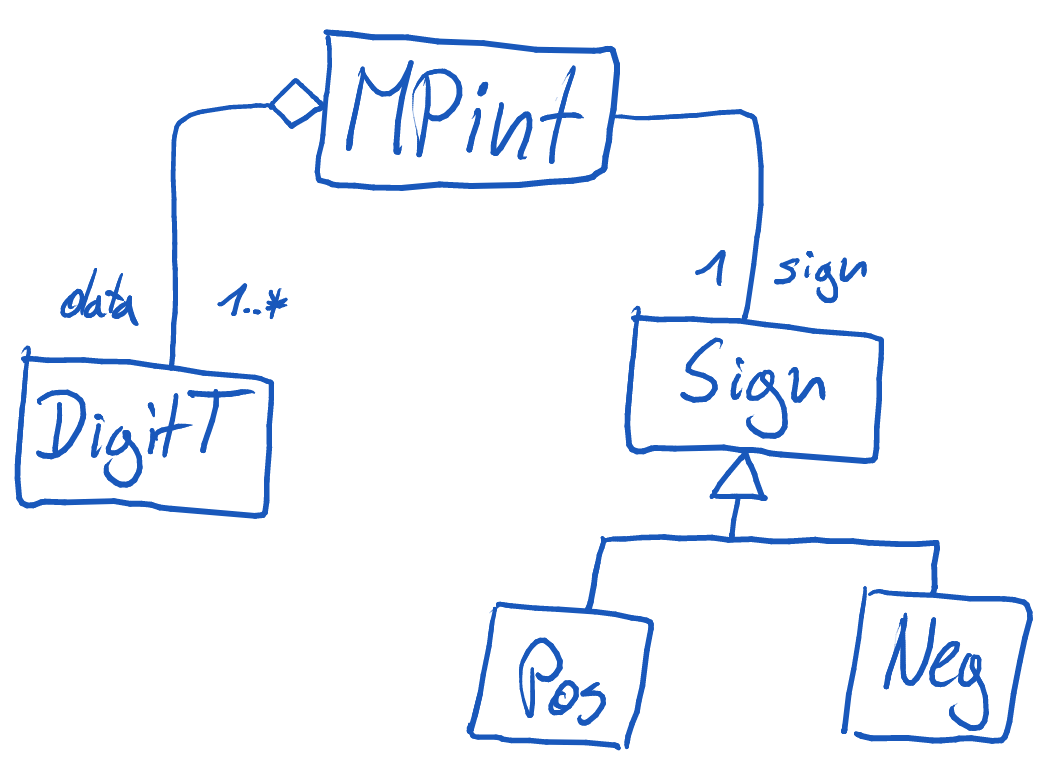
\includegraphics[width=0.5\linewidth]{images/cdmpint}
                \caption{Übersicht des \mpi\ Datentyps}
                \label{fig:cdmpint}
            \end{figure}

            Für \ilc{MPint} sind diverse \ilc{trait}s der Standardbibliothek implementiert.
            Insbesondere seien hier erwähnt:

            \begin{itemize} \tightlist
                \item die binären, arithmetischen Operatoren (\ilc{+}, \ilc{-}, \ilc{*}, \ilc{+=}),
                \item der unäre Negationsoperator (''\ilc{-x}'') und
                \item die binären Vergleichsoperatoren (\ilc{==}, \ilc{>}, \ilc{>=}, \dots)
            \end{itemize}

            Sie erlauben einen mit normalen Zahlen vergleichbaren Umgang mit den \mpi{}. Die arithmetischen Operatoren greifen dabei auf die in \autoref{sec:impldetails} angesprochenen Funktionen zurück.

            Es gibt diverse Möglichkeiten\footnote{Diese lassen sich hervorragend mit dem erwähnten Negationsoperator kombinieren, um negative \mpi\ zu erzeugen}, Instanzen zu erzeugen, u.a.:

            \begin{itemize}
                \item
                \ilc{MPint::new(u128)} \\
                    $\rightarrow$ aus nativen, vorzeichenlosen Integern
                \item
                \ilc{MPint::new(Vec<DigitT>)} bzw. Makro \ilc{mpint!(a\textsubscript{0}, a\textsubscript{1}, ...)} \\
                    $\rightarrow$ aus einer Liste an Ziffern
                \item
                \ilc{from\_hex\_str(\&str)} bzw. \ilc{from\_dec\_str(\&str)} \\
                    $\rightarrow$ aus Hex- bzw. Dezimal-Strings
            \end{itemize}

            Die \ilc{MPint::new(\dots)} Konstruktoren werden durch den benutzerdefinierten \ilc{trait}\\ \ilc{CreateNewFrom<T>} ermöglicht.

            Wie bereits erwähnt wird in Unit-Tests von Python Gebrauch gemacht. Das Vorgehen ist in zwei Phasen unterteilt:
            \begin{enumerate}
                \item Mit \ilc{mpint\_tests::verify\_arithmetic\_result(\dots)} wird die Operation und deren Ergebnis an eine Funktion in \ilc{mpint\_test\_helper.py} übergeben. Zurück kommt ein Tupel, mit der Information, ob das Ergebnis ok ist und einer passenden textuellen Meldung.

                \item Das Makro \ilc{mpint\_tests::create\_op\_correctness\_tester!} dient dazu, Code Duplikate zu vermeiden. Es erstellt für einen gegebenen Operator die entsprechend angepasste Test-Funktion. Hier ist der eigentliche \ilc{assert!} enthalten, welcher die vom Python-Skript erhaltenen Daten nutzt.
            \end{enumerate}


    \subsection{Bibliothek im eigenen Projekt nutzen} \label{sec:eigenesprojekt}
        Am Beispiel eines neuen Binary-Projekts wird jetzt gezeigt, wie sich die Bibliothek einbinden lässt.

        \paragraph*{Voraussetungen}
        Im Folgenden wird davon ausgegangen, dass Rust mit dem \href{https://rustup.rs}{\ilc{rustup}} Installer und der Standard-Toolchain eingerichtet wurde.

        \paragraph*{Schritte}

\begin{enumerate}
    \item Neues Binary-Projekt erstellen:

\begin{lstlisting}[language=bash]
cargo new my_new_project
\end{lstlisting}

    \item Library zum Projekt hinzufügen:
    \begin{itemize}
        \item \textit{Option 1} -- Direkt mit Git-Repository verknüpfen

\begin{lstlisting}[language=bash]
cd my_new_project
cargo add --git https://github.com/crochethk/mpa_project.git
\end{lstlisting}

        \item \textit{Option 2} -- Lokale Kopie nutzen
        \begin{itemize}
            \item Hole Library (z.B. Repo klonen)

\begin{lstlisting}[language=bash]
git clone https://github.com/crochethk/mpa_project.git
\end{lstlisting}

            \item Nach diesen Schritten ist die Ordnerstruktur in etwa: \\
                \begin{minipage}{10cm}
                \dirtree{%
                .1 /.
                .2 mpa\_project/.
                .2 my\_new\_project/.
                }
                \end{minipage}

            \item Verknüpfe mit lokaler Library

\begin{lstlisting}[language=bash]
cd my_new_project
cargo add --path ../mpa_project
\end{lstlisting}

        \end{itemize}
    \end{itemize}

    \item Library in \ilc{my\_new\_project} verwenden
    \begin{itemize}
        \item Inhalt von \ilc{my\_new\_project/src/main.rs} ersetzen

\begin{lstlisting}[language=Rust, style=boxed]
use mpa_lib::mp_int::*;

fn main() {
    println!("{}", mpint!(1,2));
}
\end{lstlisting}

        \item Ausführen\footnote{Ergebnis entspricht $1 \cdot (2^{64})^0 + 2 \cdot (2^{64})^1$}

\begin{lstlisting}[language=bash]
cargo run
# Out: 36893488147419103233
\end{lstlisting}


    \end{itemize}
\end{enumerate}

    \subsection{Unit-Tests ausführen}
     Aufgrund \ilc{pyo3} ist, zusätzlich zu den Voraussetzungen aus \autoref{sec:eigenesprojekt},  \href{https://pyo3.rs/main/getting-started}{mindestens eine \ilc{Python 3.7} Umgebung notwendig}.

    Um alle Tests auszuführen reicht folgender Befehl:
    \begin{lstlisting}[language=bash]
cargo test --all
    \end{lstlisting}



\section{Implementierungsdetails der Operationen} \label{sec:impldetails}
\subsection{Addition und Subtraktion}
    Da Subtraktion bezüglich Addition implementiert ist, werden beide Operationen hier gemeinsam behandelt.

    \paragraph*{Wichtige Funktionen}
        \begin{itemize} \tightlist
            \item \ilc{MPint::carry\_ripple\_add\_bins\_inplace(\&mut self, \dots) -> bool}
            \item \ilc{MPint::overflowing\_add(\&mut self, \dots) -> bool}
            \item \ilc{MPint::twos\_complement\_inplace(\&mut self)}
        \end{itemize}

    \paragraph*{Carry-Ripple-Adder}
        Prinzipiell funktioniert die implementierte Addition wie eine Reihenschaltung von ,,\ilc{u64}-Volladdierern'' (vgl. \autoref{fig:fulladderchain}).

        Die Ziffern $a_i$ und $b_i$ der Summanden $a=a_{n}a_{n-1}\dots{}a_{1}a_{0}$ und $b=b_{n}b_{n-1}\dots{}b_{1}b_{0}$ werden dabei jeweils mit Übertrag\footnote{i.A. kann bei einer Addition höchstens ein Übertrag entstehen, der genau eine Ziffer benötigt ($\hat{=}$ 1 Bit)} addiert.
        $c_i$ wird bei Addition des nächsten Ziffernpaars wieder in den Volladdierer eingespeist usw.

        Die Summe $s=a+b$ ist also:
        \begin{align*}
        s = s_{n+1}s_{n}\dots{}s_{1}s_{0} \quad
            \text{mit:} \quad
                s_i &= (a_i + b_i + c_{i-1}) \mod B \\
                c_i &= \lfloor (a_i + b_i) \div B \rfloor \\
                  B &= 2^{64}
        \end{align*}

        \begin{figure}[H]
            \centering
            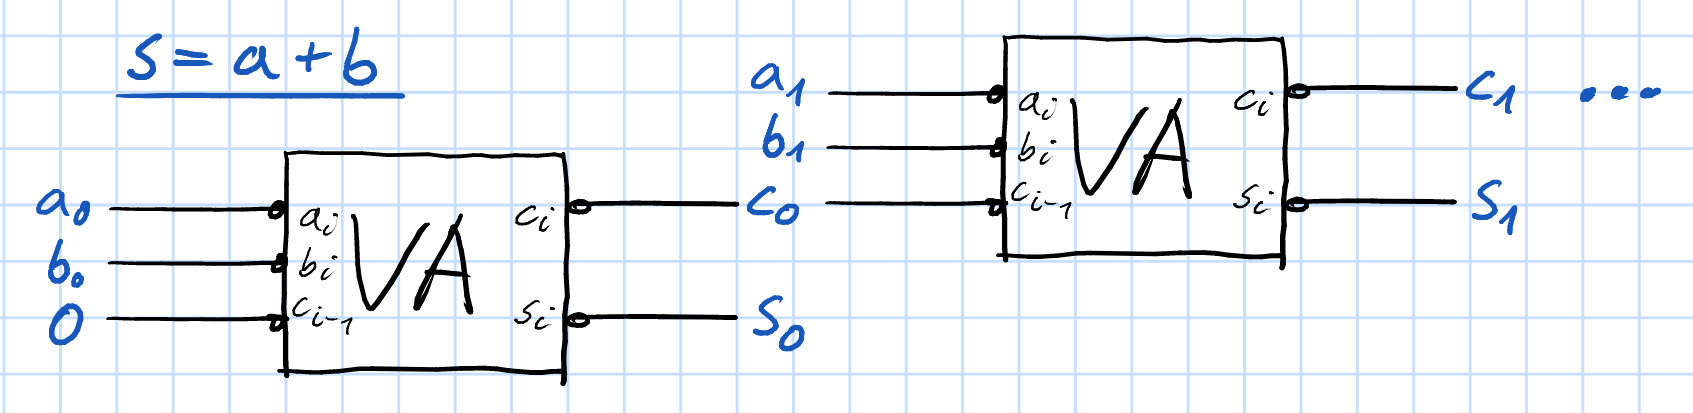
\includegraphics[width=0.7\linewidth]{images/fulladderchain}
            \caption{Addition von \mpi\ mittels Volladdierern}
            \label{fig:fulladderchain}
        \end{figure}

        Abstrakt betrachtet entspricht dieses Konzept einem sog. \emph{Carry-Ripple-Addierer}.

    \paragraph*{Gleiche Vorzeichen}
        Da intern Vorzeichen und absoluter Wert unabhängig gespeichert sind, kann die Summe bei gleichen Vorzeichen ohne Weiteres wie oben beschrieben berechnet werden.

    \paragraph*{Unterschiedliche Vorzeichen}
        Unterscheiden sich die Vorzeichen, sind weitere Schritte erforderlich. Hier tritt eine tatsächliche Subtraktion auf.


        Dank der binären Repräsentation und Eigenschaften des 2-Komplements ist es möglich die Subtraktion auf eine Addition zurückzuführen.
        Hierzu kann man zur Vereinfachung die Summanden erst einmal so ,,ordnen'', dass $b$ immer der negative und $a$ der positive Summand ist ($a \ge 0$, $b \le 0$). Man kann die Operation aufschreiben als:
        \begin{equation*}
        s = a - |b|
        \end{equation*}

        Sei nun $b^*$ das 2-Komplement von $b$, dann berechnet sich $s$ zu:

        \begin{itemize} \tightlist
            \item Falls $a \ge |b|$: (\emph{$s$ positiv})
                \begin{align*}
                    & s = a + b^*
                \end{align*}
            \item Falls $a < |b|$: (\emph{$s$ negativ})
                \begin{align*}
                    & s^* = a + b^* \\
                    & \Rightarrow s \text{ ist das 2-Komplement von } s^*
                \end{align*}
        \end{itemize}


\subsection{Multiplikation}
    Wie erwähnt wurden im Verlauf des Projekts zwei verschiedene Ansätze implementiert: \emph{Operand Scanning} und \emph{Product Scanning}.

    \subsubsection{Operand Scanning} \label{sec:opscanning}
    Dies ist der Ansatz der ersten Implemenierung, welche später durch \nameref{sec:prodscan} ersetzt wurde.
    Hierbei werden die einzelnen Ziffern der \emph{Operanden} miteinander zu Teilprodukten und Überträgen multipliziert. Anschließend wird alles entsprechend des jeweiligen Stellenwerts zum Gesamtergebnis (Produkt) addiert (vgl. \autoref{fig:opscanning}).

    Der Vollständigkeit halber ist der entsprechende Code als \autoref{apdx:opscan} inkludiert.
    Im Vergleich zum nachfolgenden Ansatz, fällt dort auf, dass u.a. zwei 2D-Matrizen für Zwischenergebnisse und mehrfaches Iterieren benötigt wurden.

    \begin{figure}[H]
        \centering
        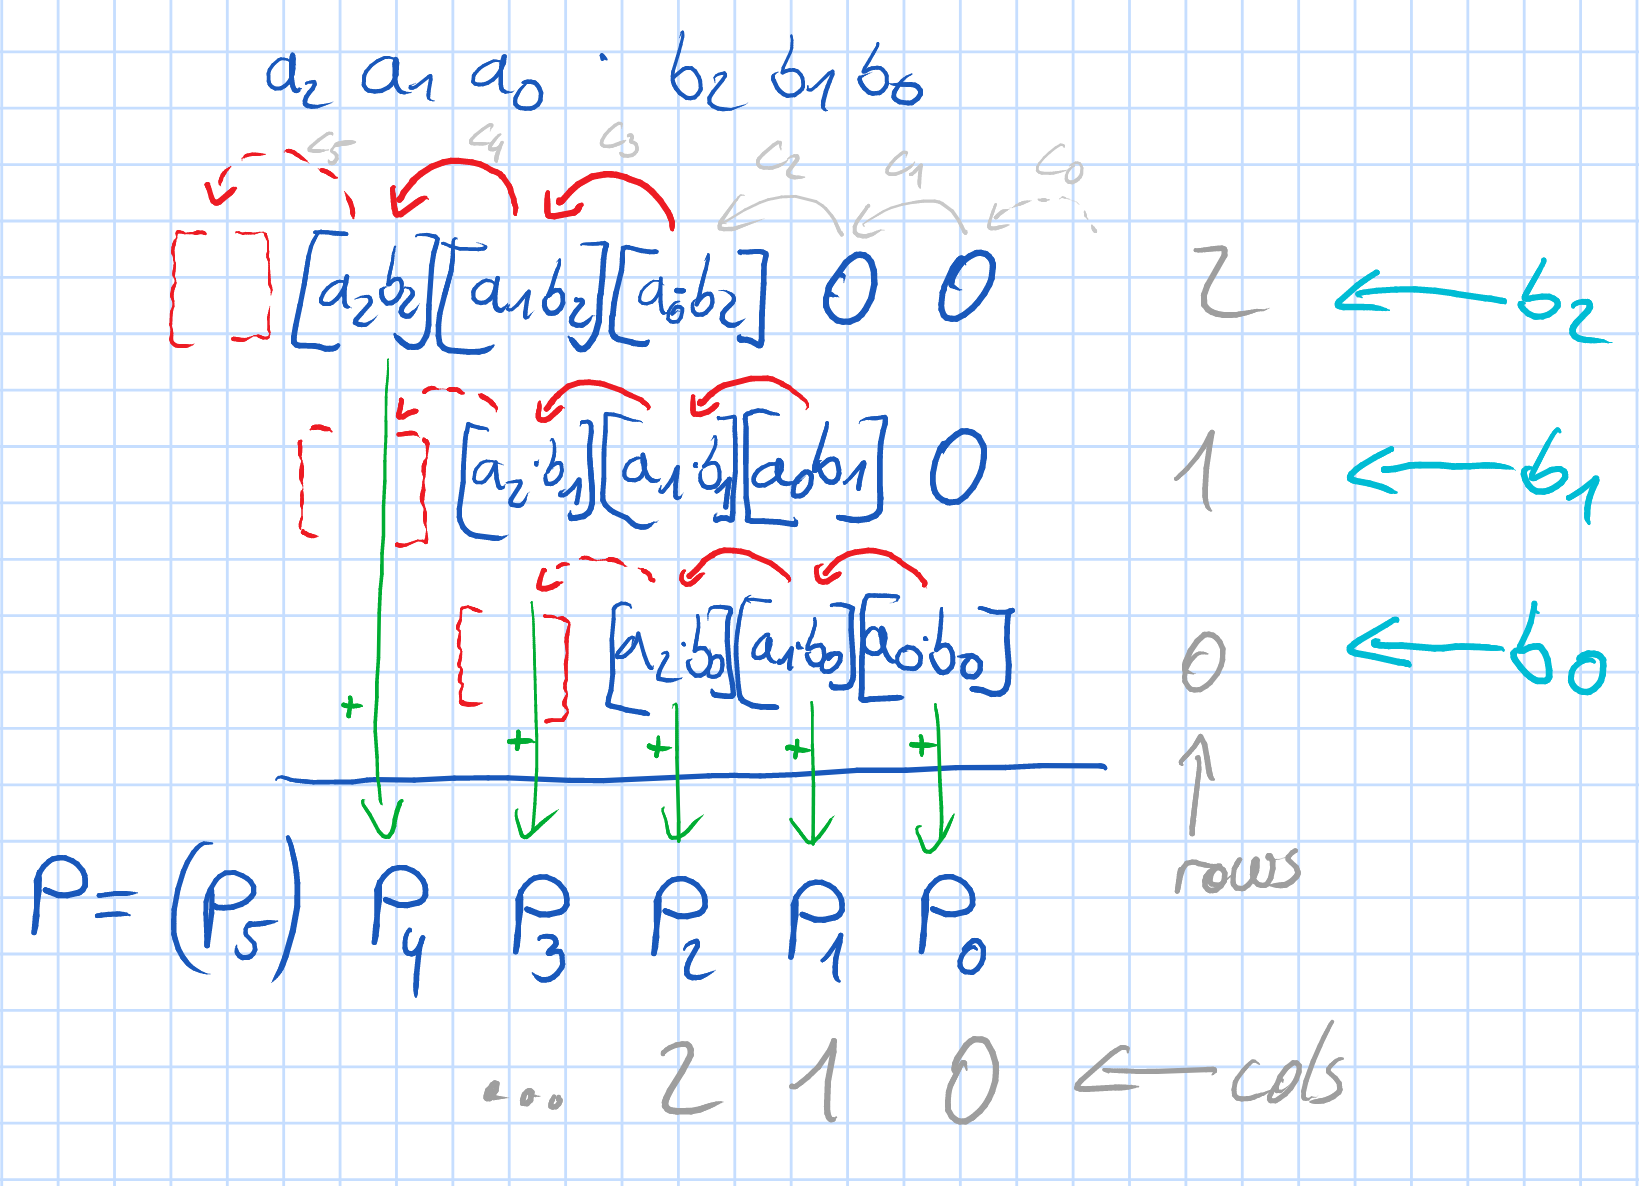
\includegraphics[width=0.7\linewidth]{images/opscanning}
        \caption{Veranschaulichung des Operand Scanning Ansatzes}
        \label{fig:opscanning}
    \end{figure}

\subsubsection{Product Scanning} \label{sec:prodscan}

    \paragraph*{Wichtige Funktionen}
    \begin{itemize} \tightlist
        \item Addition (s.o.)
        \item \ilc{MPint::prod\_scan\_mul(\&self, \dots) -> Self}
    \end{itemize}

    \paragraph*{Erklärung}
    Dieser Ansatz erspart das Vorhalten aller Teilprodukte und Überträge während der Berechnung. Stattdessen werden die einzelnen Produkt-Ziffern eine nach der anderen, \emph{direkt} berechnet.

    Das funktioniert deshalb, weil Ziffern der Operanden nur einen beschränkten Einflussbereich auf Ziffern des Produkts haben (vgl. \autoref{fig:prodscanningeinfluss}). Beispielsweise wird die erste Ziffer des Produkts ausschließlich von den beiden ersten Ziffern der Operanden beeinflusst. Bei der letzten Ziffer des Produkts verhält es sich analog, nur dass evtl. ein Übertrag aus den vorherigen Ziffern einfließt. Dementsprechend muss man von ,,rechts nach links'' durch das Produkt iterieren.

    Dabei betrachtet der implementierte Algorithmus die Operanden als hätten sie gleich vielen Ziffern und füllt bei unterschiedlicher Anzahl ggf. den ,,kürzeren'' Operand links mit Nullen auf.

    Seien $a=a_{n}a_{n-1}\dots{}a_{1}a_{0}$ und $b=b_{n}b_{n-1}\dots{}b_{1}b_{0}$ die beiden Operanden.
    Da das Produkt $p = a \cdot b$ zweier Zahlen mit jeweils $n$ Ziffern höchstens $2 \cdot n$ Ziffern haben kann, gilt $p=p_{2n}p_{2 n-1}\dots{}p_{1}p_{0}$.

    Seien nun $i$ der Index, mit dem die einzelnen Ziffern des Produkts
    und $j$ der Index, mit dem die Ziffern beider Operanden referenziert werden.

    Aus besagtem Einflussbereich ergibt sich folgender Algorithmus zur Berechnung der einzelnen Produkt-Ziffern:
    \begin{enumerate}
        \item Sei $k=i-j$:
            \begin{itemize} \tightlist
                \item Falls $k \ge n$: Überspringe die aktuelle Operand-Ziffer ($j$)
                \item Falls $k < 0$: Ende des Einflussbereichs wurde erreicht. Gehe zur nächsten Produkt-Ziffer ($i$)
            \end{itemize}

        \item Die $i$-te Produkt-Ziffer $p_i$ wird berechnet als:
            \begin{itemize} \tightlist
                \item Summe aller Teilprodukte $p_{i,j} = a_j \cdot b_k$, wobei jedes offensichtlich bis zu 2 Ziffern ergeben kann (\ilc{u64 $\rightarrow$ u128})
                \item Addition des letzten Übertrags $c_{i-1}$
                \item Anschließende Modulo-Berechnung zur Basis des Zahlensystems.
            \end{itemize}
        \item Berechnen des Übertrags $c_{i}$ für die folgende Ziffer, als Quotient\footnote{Statt tatsächlich zu dividieren, wird hier einfach die ,,MSB-Hälfte'' der Bits des Zwischenergebnisses genommen.} aus  der obigen Gesamtsumme (vor Modulo-Berechnung).
    \end{enumerate}

    \begin{figure}[H]
        \centering
        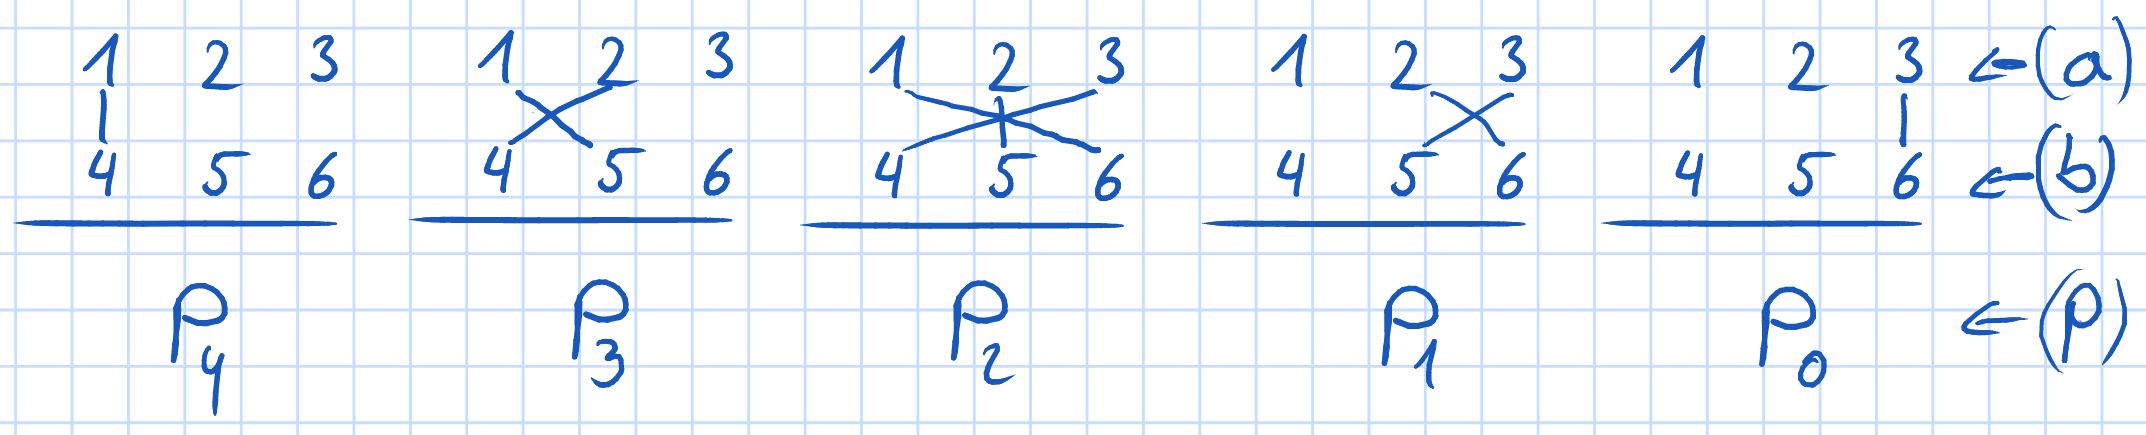
\includegraphics[width=0.7\linewidth]{images/prodscanningeinfluss}
        \caption{Veranschaulichung des Einflussbereichs der Ziffern beim Product Scanning Ansatz. $a$ und $b$ sind die Operanden, $p$ das Produkt. Die Linien zeigen, welche Ziffern in die jeweilige Produkt-Ziffer \emph{direkt} einfließen}
        \label{fig:prodscanningeinfluss}
    \end{figure}



\section{Extras}\label{sec:extras}

\subsection{\ilc{rustdoc}}
Wie bereits erwähnt ist der Quellcode ausführlich mittels \emph{doc comment}s dokumentiert.
Mit folgendem Befehl lässt sich daraus eine HTML-Dokumentation in gewohnter ,,Rust-Optik'' generieren, welche im Anschluss unter \ilc{target/doc} zu finden ist:

\begin{lstlisting}[language=bash]
cargo doc --no-deps --examples --bins

# Alternativ: Inklusive privater Elemente
cargo doc --no-deps --examples --bins --document-private-items
\end{lstlisting}

\subsection{Demo CLI}
Dies ist die Standard-Anwendung, welche beim Aufruf von \ilc{cargo run} ausgeführt wird.
Es gibt zwei Modi:
\begin{itemize}
    \item Zum einen kann man eine Anzahl \textbf{zufälliger Testoperationen} ausführen und diese auf Wunsch inkl. des Ergebisses in einer Textdatei speichern lassen. Dabei ist das Format\footnote{Pro Zeile: \ilc{\{lhs\}\{operator\}\{rhs\}==\{mpa\_lib Ergebnis\}}} so gewählt, dass der komplette Inhalt direkt in eine Python Shell eingefügt werden kann, worauf automatisch alle Ergebnisse mit Pythons Ergebnissen verglichen werden.

    \item Zum anderen gibt es einen \textbf{interaktiven Modus}, der eine einfache REPL\footnote{read-evaluate-print-loop} bietet.
\end{itemize}

Eine ausführliche Beschreibung ist im Quellcode (\ilc{src/bin/mpa\_demo\_cli.rs}) bzw. als \ilc{rustdoc} (s. o.) verfügbar.

Vefügbare Optionen können zudem angezeigt werden mittels
\begin{lstlisting}[language=bash]
cargo run -- --help
\end{lstlisting}


\subsection{Examples}
Im Ordner \ilc{examples} sind folgende Beispiel Anwendungen der Bibliothek vorhanden:

\begin{minipage}{10cm}
    \dirtree{%
        .1 examples/.
        .2 binomial.rs.
        .2 exponentiation.rs.
        .2 simple\_factorial.rs.
    }
\end{minipage}

Um eines der Beispiele auszuführen kann man folgenden Befehl benutzen:

\begin{lstlisting}[language=bash]
cargo run --example binomial
\end{lstlisting}

Zum Teil beinhalten die Beispiele auch Unit-Tests, welche nicht zusammen mit den normalen Tests der Bibliothek aufgerufen werden. Sie können aber manuell wie folgt ausgeführt werden:

\begin{lstlisting}[language=bash]
cargo test --example binomial

# bzw. alle auf einmal:
cargo test --examples
\end{lstlisting}

\section{Future Works}
Auch wenn die Bibliothek an sich die geforderte Funktionalität erfüllt, kann sie selbstverständlich an vielen Stellen weiter verbessert werden.
Neben Vereinheitlichung der öffentlichen Schnittstelle seien hier insbesondere die Implementierung effizienterer Multiplikations-Algorithmen (z.B. emph{Karazuba}) und modularer Multiplikation (z.B. emph{Montgomery-Multiplikation}) erwähnt. Letztere ist gerade in der Kryptografie von großer Bedeutung.
Des Weiteren ist zur Performance-Steigerung der Multiplikation denkbar, \emph{SIMD}-Fähigkeiten des Prozessors auszunutzen -- z.B. zur Berechnung aller Teilprodukte in einem Schritt statt nacheinander.



\appendix
\section{Operand Scanning Code} \label{apdx:opscan}
\begin{lstlisting}[language=Rust, style=boxed]
    /// Multiplies two `MPint`, extending the width as necessary.
    /// This uses a kind of "Operand-Scanning" algorithm.
    fn extending_operand_scan_mul(&self, rhs: &Self) -> Self {
        self.assert_same_width(rhs);

        // Zero short circuit
        if self.is_zero() {
            return self.clone();
        } else if rhs.is_zero() {
            return rhs.clone();
        }

        let result_sign = if self.sign == rhs.sign {
            // same signs implicate positive result
            Sign::Pos
        } else {
            // different signs implicate negative result
            Sign::Neg
        };
        let max_new_width = self.width * 2;

        // ~~~~ Main ~~~~

        // Given `a*b = a0..an * b0..bn` where `a0..an` and `b0..bn` are the digits of the factors.
        // Each row of following matrices represents the multiplication of a digit of one factor
        // with each digit of the other factor, with offset of the first factors digit-position.

        // Matrix with: "digits_count" rows and "2*digits" columns
        let mut prod_rows = vec![vec![0 as DigitT; self.len() * 2]; self.len()];

        // `prod_carries[i][j]` represents the carry, which resulted from multiplying the i-th digit
        // of one factor by the (j-1)-th digit of the other factor. This carry must then be added to
        // the j-th digit of the end result.
        // First column of carries is always zero.
        let mut prod_carries = vec![vec![0 as DigitT; self.len() * 2]; self.len()];

        for i in 0..prod_rows.len() {
            let b_i = rhs[i] as DoubleDigitT;

            for j in 0..self.len() {
                let a_j = self[j] as DoubleDigitT;
                let prod_ij = a_j * b_i;

                prod_rows[i][j + i] = prod_ij as DigitT;
                prod_carries[i][j + i + 1] = (prod_ij >> DIGIT_BITS) as DigitT;
            }
        }

        // Sum columns

        let mut end_product = MPint::new(max_new_width);
        let mut col_carry = 0 as DigitT;
        for j in 0..prod_rows[0].len() {
            // Add last columns carry
            end_product += col_carry;

            for i in 0..prod_rows.len() {
                col_carry = end_product.carry_ripple_add_bins_inplace(&MPint::from_digit(
                prod_rows[i][j],
                max_new_width,
                )) as u64;

                col_carry += end_product.carry_ripple_add_bins_inplace(&MPint::from_digit(
                prod_carries[i][j],
                max_new_width,
                )) as u64;
            }

            // Make sure next column is added to the correct position of the number system
            end_product.rotate_digits_right(1);
        }

        // ~~~~ Epilog ~~~~
        end_product.trim_empty_end(self.len());
        end_product.sign = result_sign;

        end_product
    }
\end{lstlisting}

\end{document}
